%% --------------------------------------------------------------
%%
%% I N T R O D U C T I O N
%%
%% --------------------------------------------------------------
\section{Introduction}
\begin{frame}{}  %% ---------- Intro/motivation 
    \begin{tikzpicture}[overlay,remember picture]
        
        \uncover<1->{ % <-> |
            \node (t1) [anchor=center,scale=1,opacity=1] at ([shift={(-3.5cm,-0.5cm)}]current page.center){
                \parbox{0.6\textwidth}{
                    \begin{itemize}
                        \item One of the ways to understand the properties of matter at supernuclear densities 
                        is to study EM signatures of BNS, NSBH mergers and CCSNe. 
                        %
                        \item Non-thermal EM signatures: GRBs, kN afterglows, ... 
                        %
                        \item Origin: interaction between transrelativistic ejecta and ISM. 
                        %
                        \item Thus study of GRBs, kN probe the ejecta properties and by extension, the 
                        properties of the postmerger/post-SNe remnant. 
                        \item NR simulations + observations show 
                    \end{itemize}
            }};
            
        }
        
%        \uncover<1->{ % <-> |
%            \node (t1) [anchor=center,scale=1,opacity=1] at ([shift={(-3.5cm,-2.4cm)}]current page.center){
%                \parbox{0.6\textwidth}{
%                    \begin{itemize}
%                        \item Kilonova: decay of $r$-process elements. Days-Weeks.
%                        \item Afterglow: synchrotron emission from shocked ISM. Weeks-Years. 
%                    \end{itemize}
%            }};
%        }
        
        \uncover<1-1>{ % <-> |
            \node (img1) [anchor=center,scale=1,opacity=1] at ([shift={(5.6cm,-0.8cm)}]current page.center){
                \parbox{0.5\textwidth}{
                    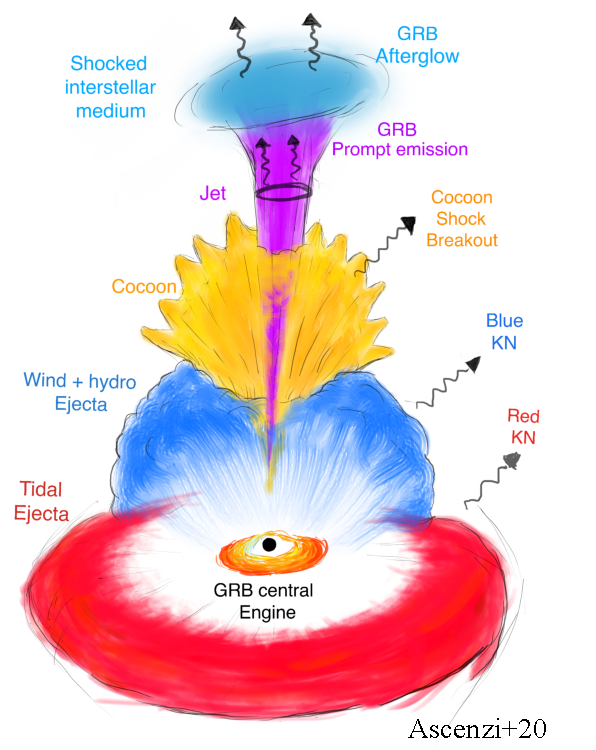
\includegraphics[height=7.0cm]{figures/Ascenzi20_EjectaEMPicture.pdf}
                    
                    %\small{\textbf{Artist depiction of ejecta$^\text{\citep{Ascenzi:2020xqi}}$}}
            }};
        }
    \end{tikzpicture}
\end{frame}

%                    \begin{itemize}
%    \item Electrons, moving in a magnetic field emit "curavature" radiation. 
%    \item Relativistic (non-relativistic) electrons emit synchrotron (cyclotron)
%    \item Both limits can be treated analytically. Trnasion -- cannot. 
%    \item Cyclotron emission is common in solar flare modelling. 
%    %                        \item If magnetic fields are very strong, cyclotron harmonics develope fine structure. 
%    \item (i) Neglecting quantum effects. 
%    \item Cyclotron radiation: observer sees specturm composed of delta factions at $\omega_0$; % orbital frequency.
%    \item As electron speeds up: observer sees additional Fourier components (harmonics), $\omega_0 \propto \gamma_e^{-1}$, emission becomes more beamed in the direction of motion. 
%    \item For a realtivistc electron: spectrim is a close series of delta functions (continous) 
%    up to $\omega \sim \omega_{b}\gamma_e^2$ with universal shape. % cyclotron frequency $omega_b = eB/m_ec$
%\end{itemize}

% =============================================================================================
\section{GRB afterglow}
\begin{frame}{}  %% ---------- Intro/motivation 
    \begin{tikzpicture}[overlay,remember picture]
        \uncover<1->{ % <-> |
            \node (t1) [anchor=center,scale=1,opacity=1] at ([shift={(-3.5cm,-0.5cm)}]current page.center){
                \parbox{0.6\textwidth}{
                    \begin{itemize}
                        \item Short vs Long but Uncertain origin.
                        %
                        \item Generally display three main stages: Thermal/photosphere; prompt; afterglow
                        %
                        \item Afterglow: synchrotron emission from forward shock (reverse?). 
                        %
                        \item Difeverse afterglow-scape: plateus, flares, shallow rise, rebrightening(?)
                        \item NR simulations + observations show 
                    \end{itemize}
                    Difeverse afterglow-scape: plateus, flares, shallow rise, rebrightening(?)
                    $\rightarrow$ central enigine activity. 
                    (Reverse shock probes jet properties Poynting flux/baryon dominated)
                    %
                    Example: GRB170817A, sGRB from BNS merger. 
                    Afterglow modelling $\rightarrow$ contraints on inclanation angle. 
            }};
            
        }
        
        %        \uncover<1->{ % <-> |
            %            \node (t1) [anchor=center,scale=1,opacity=1] at ([shift={(-3.5cm,-2.4cm)}]current page.center){
                %                \parbox{0.6\textwidth}{
                    %                    \begin{itemize}
                        %                        \item Kilonova: decay of $r$-process elements. Days-Weeks.
                        %                        \item Afterglow: synchrotron emission from shocked ISM. Weeks-Years. 
                        %                    \end{itemize}
                    %            }};
            %        }
        
        \uncover<1-1>{ % <-> |
            \node (img1) [anchor=center,scale=1,opacity=1] at ([shift={(4.5cm,1.4cm)}]current page.center){
                \parbox{0.5\textwidth}{
                    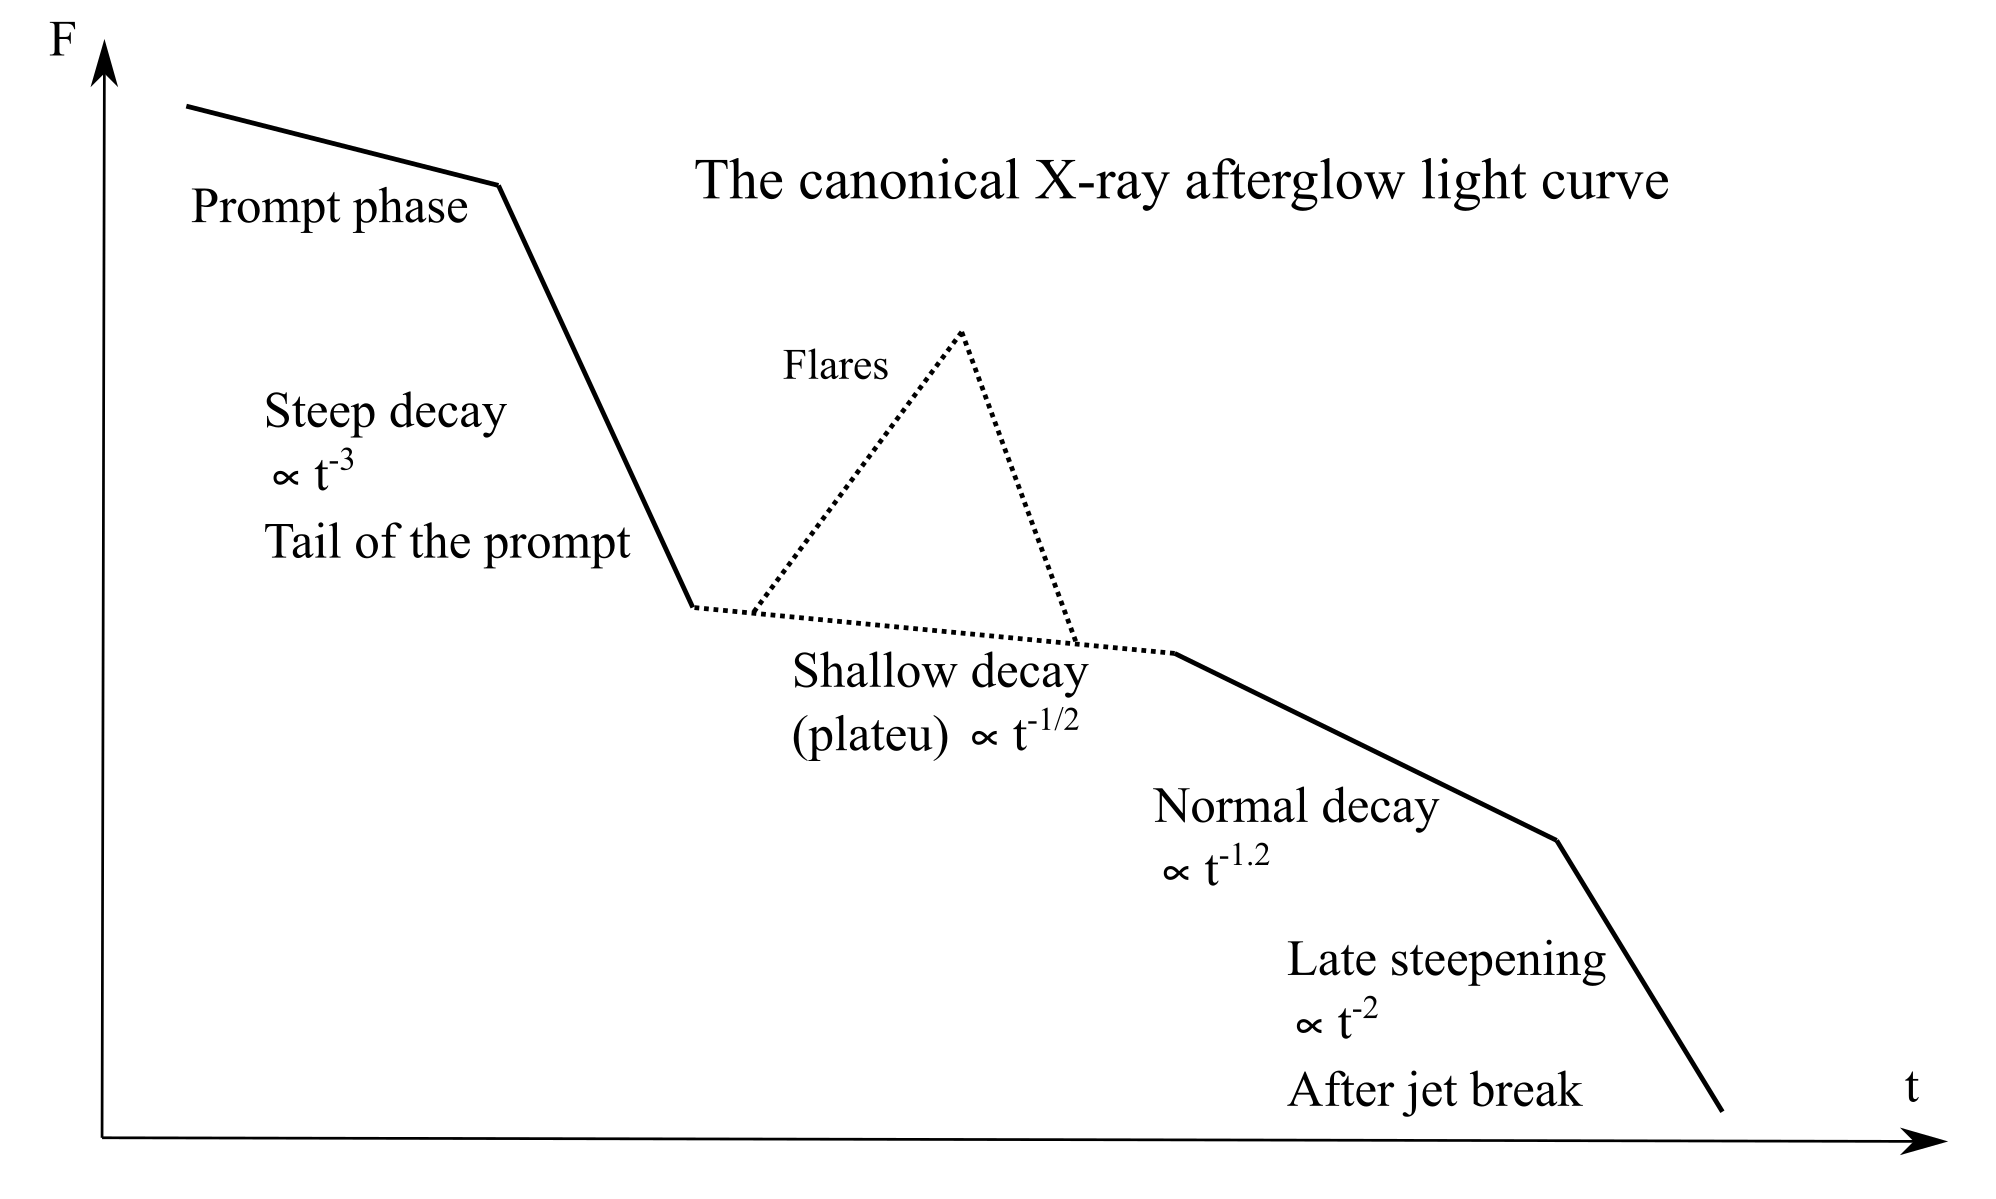
\includegraphics[height=4.2cm]{figures/grb_xray_canonic.png}
                    
                    %\small{\textbf{Artist depiction of ejecta$^\text{\citep{Ascenzi:2020xqi}}$}}
            }};
        }
        \uncover<1-1>{ % <-> |
            \node (img1) [anchor=center,scale=1,opacity=1] at ([shift={(5.0cm,-2.4cm)}]current page.center){
                \parbox{0.5\textwidth}{
                    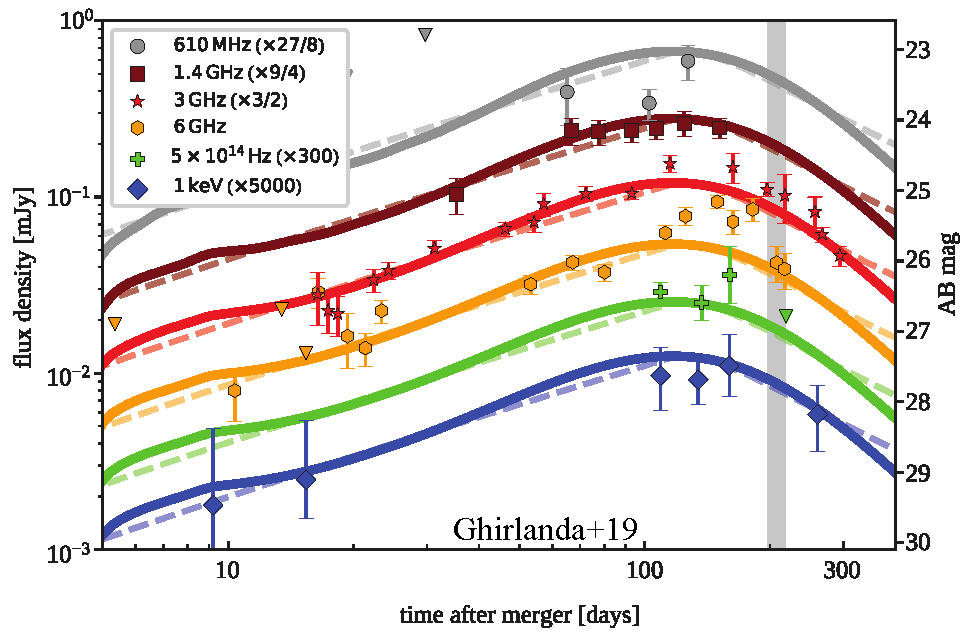
\includegraphics[height=3.8cm]{figures/Ghirlanda19_GRB170817A.pdf}
                    
                    %\small{\textbf{Artist depiction of ejecta$^\text{\citep{Ascenzi:2020xqi}}$}}
            }};
        }
    \end{tikzpicture}
\end{frame}


% =============================================================================================
\section{kN afterglows}
\begin{frame}{}  %% ---------- Intro/motivation 
    \begin{tikzpicture}[overlay,remember picture]
        \uncover<1->{ % <-> |
            \node (t1) [anchor=center,scale=1,opacity=1] at ([shift={(-3.5cm,-0.5cm)}]current page.center){
                \parbox{0.6\textwidth}{
                    \begin{itemize}
                        \item Phenomenologically similar to SNe remnants (emission from the shocks formed as ejecta speeps up ISM)
                        %
                        \item Theoretically predicted but so far unobserved (ish)
                        %
                        \item Gives info on the fastests ejecta from mergers (thus tracing dynamics in the strong-field regime)
                        %
                        \item Radial/lateral structure $\rightarrow$ diverse light curves
                        \item Complex spectra as different electron populations play role
                    \end{itemize}
                    Importantly: follows the GRB -- non-trivial interaction. 
            }};
            
        }
        %        
        %        \uncover<1->{ % <-> |
            %            \node (t1) [anchor=center,scale=1,opacity=1] at ([shift={(0.0cm,-3.8cm)}]current page.center){
                %                \parbox{1.1\textwidth}{
                    %                    \red{Questions}: remnant's lifetime; ejecta properties; \rproc{} cites
                    %            }};
            %        }
        \uncover<1-1>{ % <-> |
            \node (img1) [anchor=center,scale=1,opacity=1] at ([shift={(5.0cm,1.8cm)}]current page.center){
                \parbox{0.5\textwidth}{
                    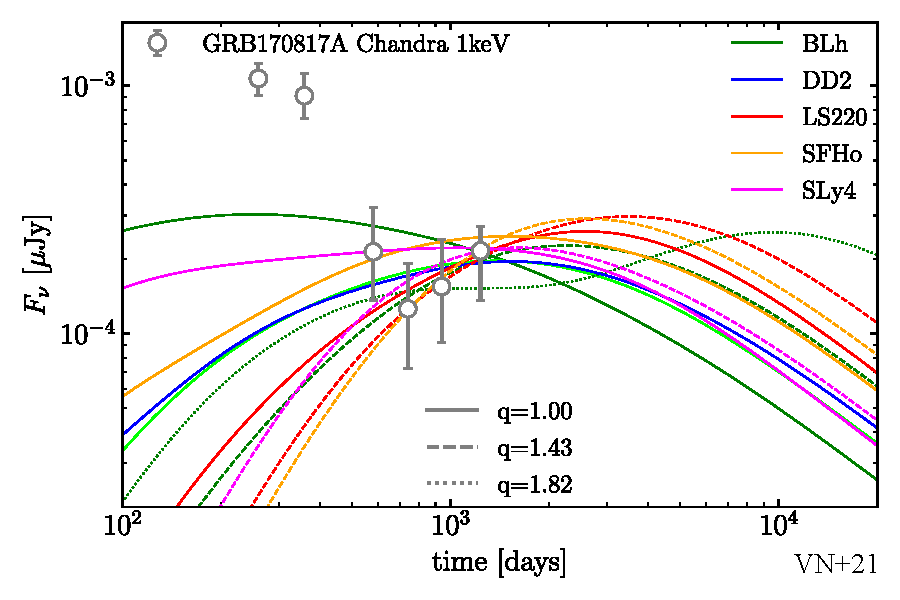
\includegraphics[height=3.8cm]{figures/best_xray_obs_representative_all_eos.pdf}
                    
                    %\small{\textbf{Artist depiction of ejecta$^\text{\citep{Ascenzi:2020xqi}}$}}
            }};
        }
        \uncover<1-1>{ % <-> |
            \node (img1) [anchor=center,scale=1,opacity=1] at ([shift={(5.2cm,-2.2cm)}]current page.center){
                \parbox{0.5\textwidth}{
                    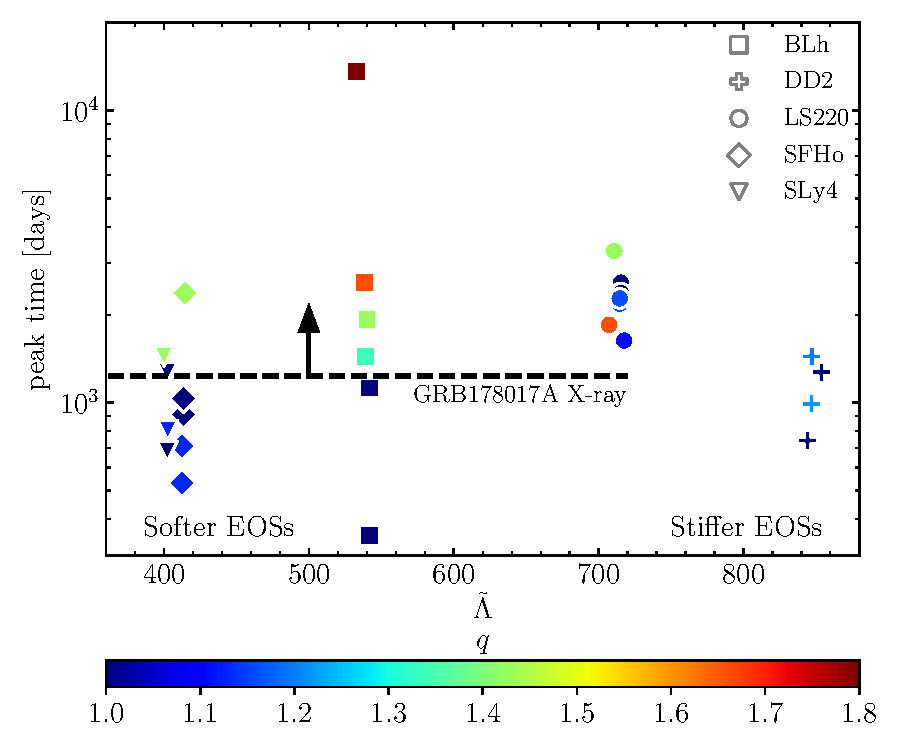
\includegraphics[height=4.2cm]{figures/scatter_lightcurve_tpeak_vs_lambda.pdf}
                
                %\small{\textbf{Artist depiction of ejecta$^\text{\citep{Ascenzi:2020xqi}}$}}
            }};
        }
    \end{tikzpicture}
\end{frame}


% =============================================================================================

\section{Geometry}
\begin{frame}{}  %% ---------- Intro/motivation 
    \begin{tikzpicture}[overlay,remember picture]
        \uncover<1->{ % <-> |
            \node (t1) [anchor=center,scale=1,opacity=1] at ([shift={(-3.5cm,-0.5cm)}]current page.center){
                \parbox{0.6\textwidth}{
                    \begin{itemize}
                        \item Numerical semi-analytic model of a 
                        \item (i) laterally structured GRB jet and 
                        \item (ii) laterally-radially structured kilonova ejecta,
                        \item expanding into GRB-evacuated ISM.
                    \end{itemize}
                    Importantly: follows the GRB -- non-trivial interaction. 
            }};
            
        }
        %        
        %        \uncover<1->{ % <-> |
            %            \node (t1) [anchor=center,scale=1,opacity=1] at ([shift={(0.0cm,-3.8cm)}]current page.center){
                %                \parbox{1.1\textwidth}{
                    %                    \red{Questions}: remnant's lifetime; ejecta properties; \rproc{} cites
                    %            }};
            %        }
        \uncover<1-1>{ % <-> |
            \node (img1) [anchor=center,scale=1,opacity=1] at ([shift={(5.5cm,-0.0cm)}]current page.center){
                \parbox{0.5\textwidth}{
                    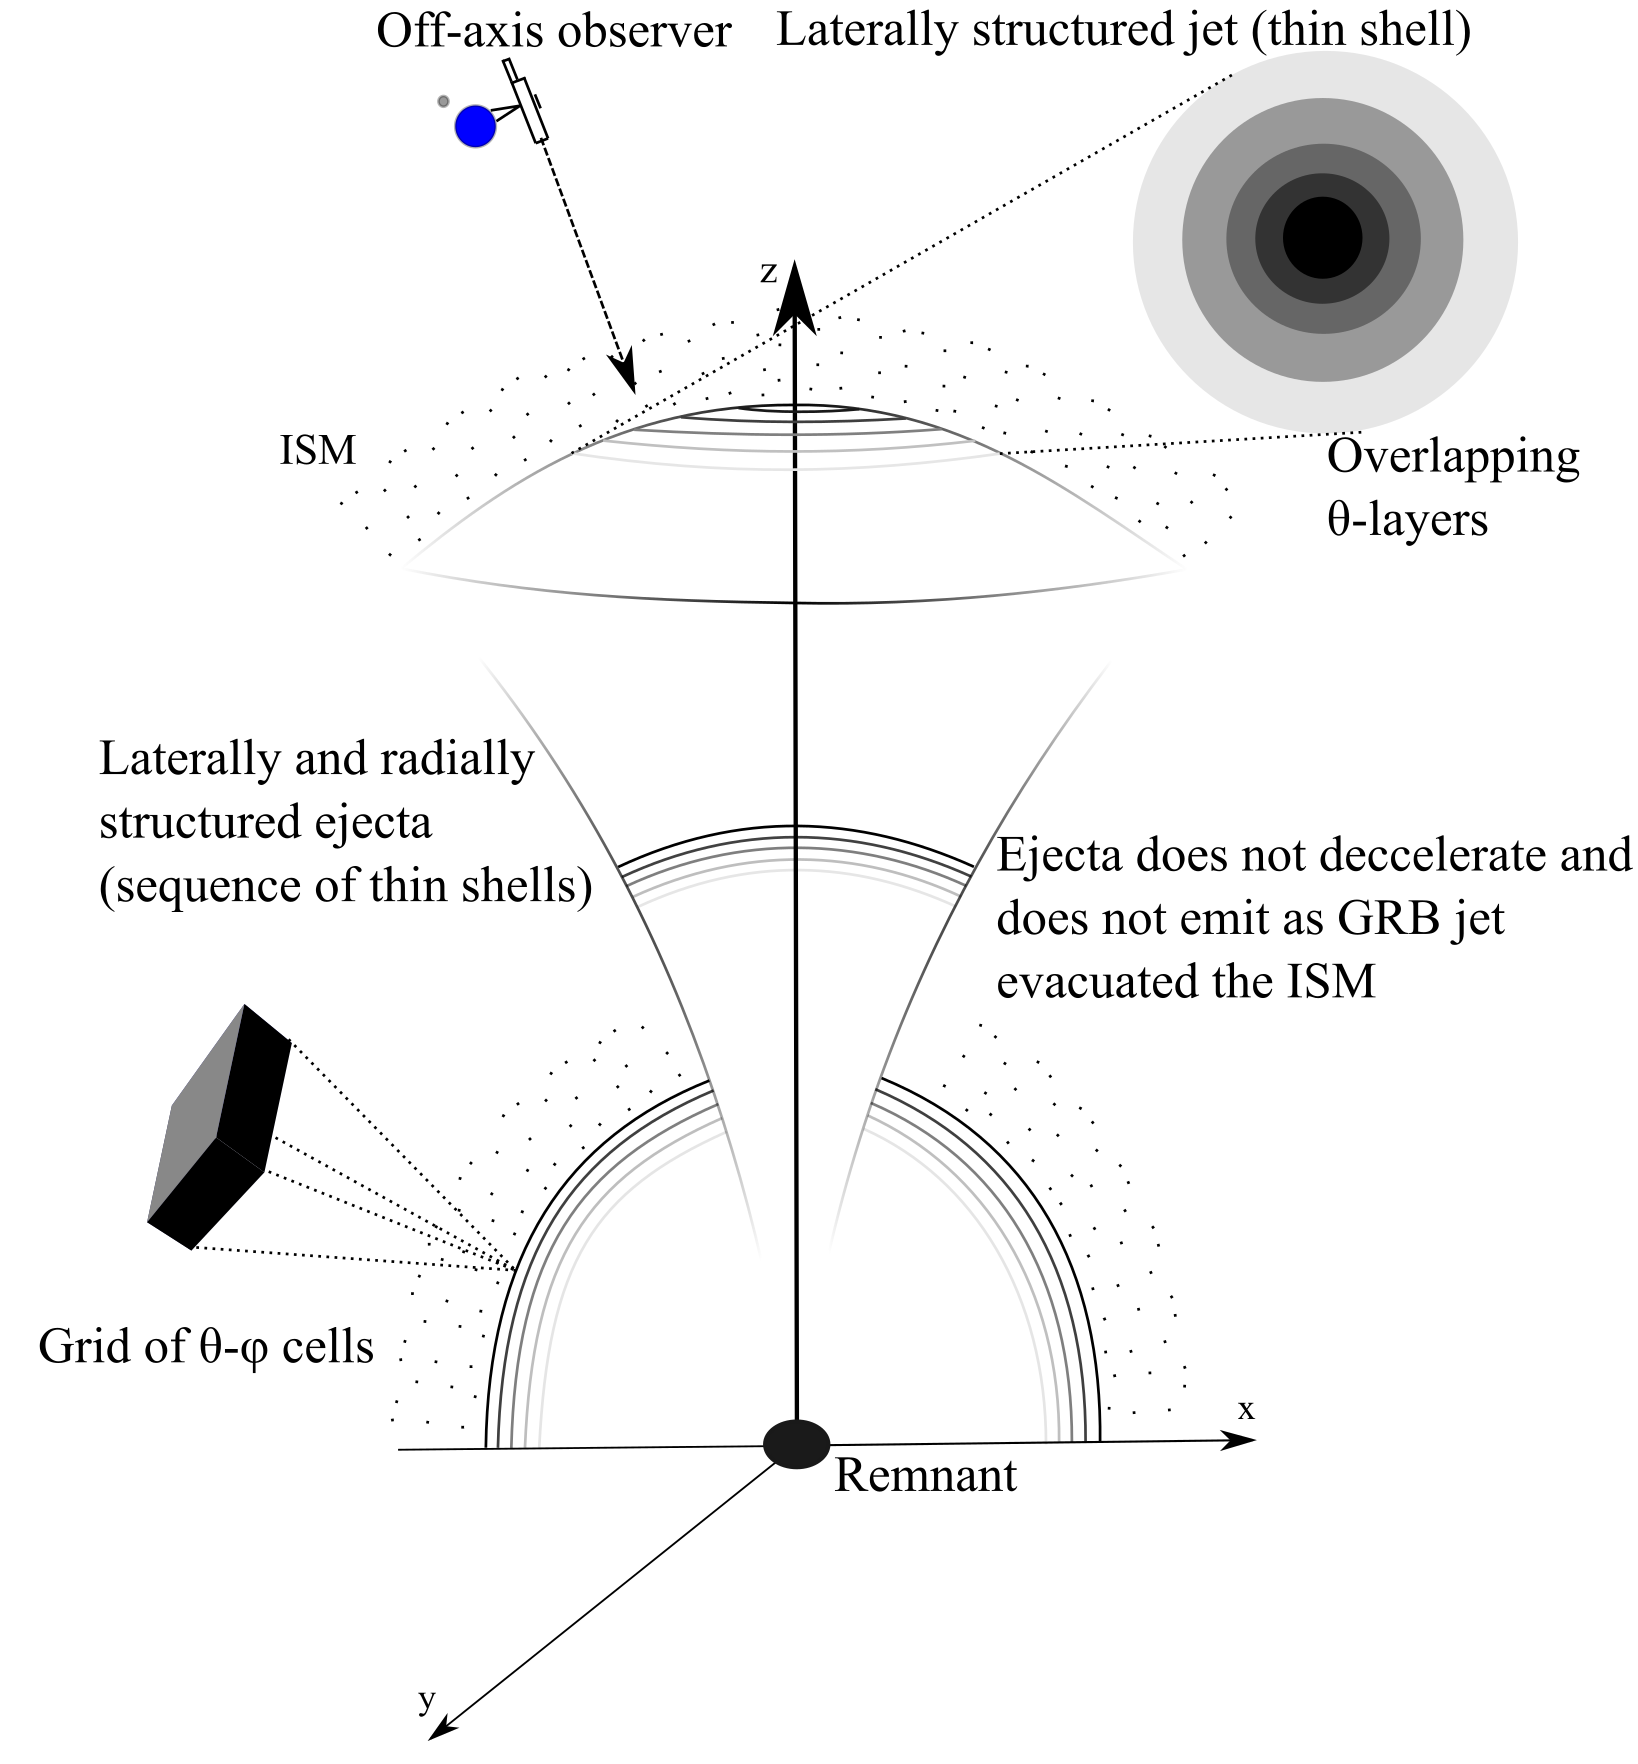
\includegraphics[height=6.0cm]{figures/structure.png}
                    
                    %\small{\textbf{Artist depiction of ejecta$^\text{\citep{Ascenzi:2020xqi}}$}}
            }};
        }
    \end{tikzpicture}
\end{frame}



% =============================================================================================

\section{Phsyics}
\subsection{Dynamics}
\begin{frame}{}  %% ---------- Intro/motivation 
    \begin{tikzpicture}[overlay,remember picture]
        \uncover<1->{ % <-> |
            \node (t1) [anchor=center,scale=1,opacity=1] at ([shift={(-3.5cm,-0.5cm)}]current page.center){
                \parbox{0.6\textwidth}{
                    Blast wave dynamics under ``thin-shell'' approximation. 
                    \begin{itemize}
                        \item jet/ejection duration is short (ejecta thickness is small)
                        \item $E_{\rm kin} \gg e_{\rm th}, p$
                        \item $4$ region system 
                    \end{itemize}
                    \begin{equation*}
                        E = \Gamma M_{0} c^2 + T^{00}V, \hspace{2mm}
                        T^{00} = (\epsilon' + P')\Gamma - P'
                    \end{equation*}
                    \begin{equation*}
                        P' = (4/3)(\Gamma^2-1)\rho c^2, \hspace{2mm}
                        \rho' = 4\Gamma\rho, \hspace{2mm}
                        \epsilon' = 4\Gamma\rho c^2
                    \end{equation*}
                    After $dt$, blast-wave speeps up $dm$ 
                    from ISM, and energy consiervation gives $d\Gamma$.
                    Separate presciption for spreading $d\theta/dt$. 
            }};
        }
        \uncover<1->{ % <-> |
            \node (t1) [anchor=center,scale=1,opacity=1] at ([shift={(4.2cm,-2.0cm)}]current page.center){
                \parbox{0.5\textwidth}{
                    Turbulent magnetic fields in the shock downstream \& first order Fermi acceleration
                    \begin{itemize}
                        \item Equipartition parameters $\varepsilon_e$, $\varepsilon_B$
                        \item first order Fermi acceleration of electrons
                        \item Non-thermal (thernal) electron population
                    \end{itemize}
            }};
        }
        \uncover<1-1>{ % <-> |
            \node (img1) [anchor=center,scale=1,opacity=1] at ([shift={(4.0cm,2.0cm)}]current page.center){
                \parbox{0.5\textwidth}{
                    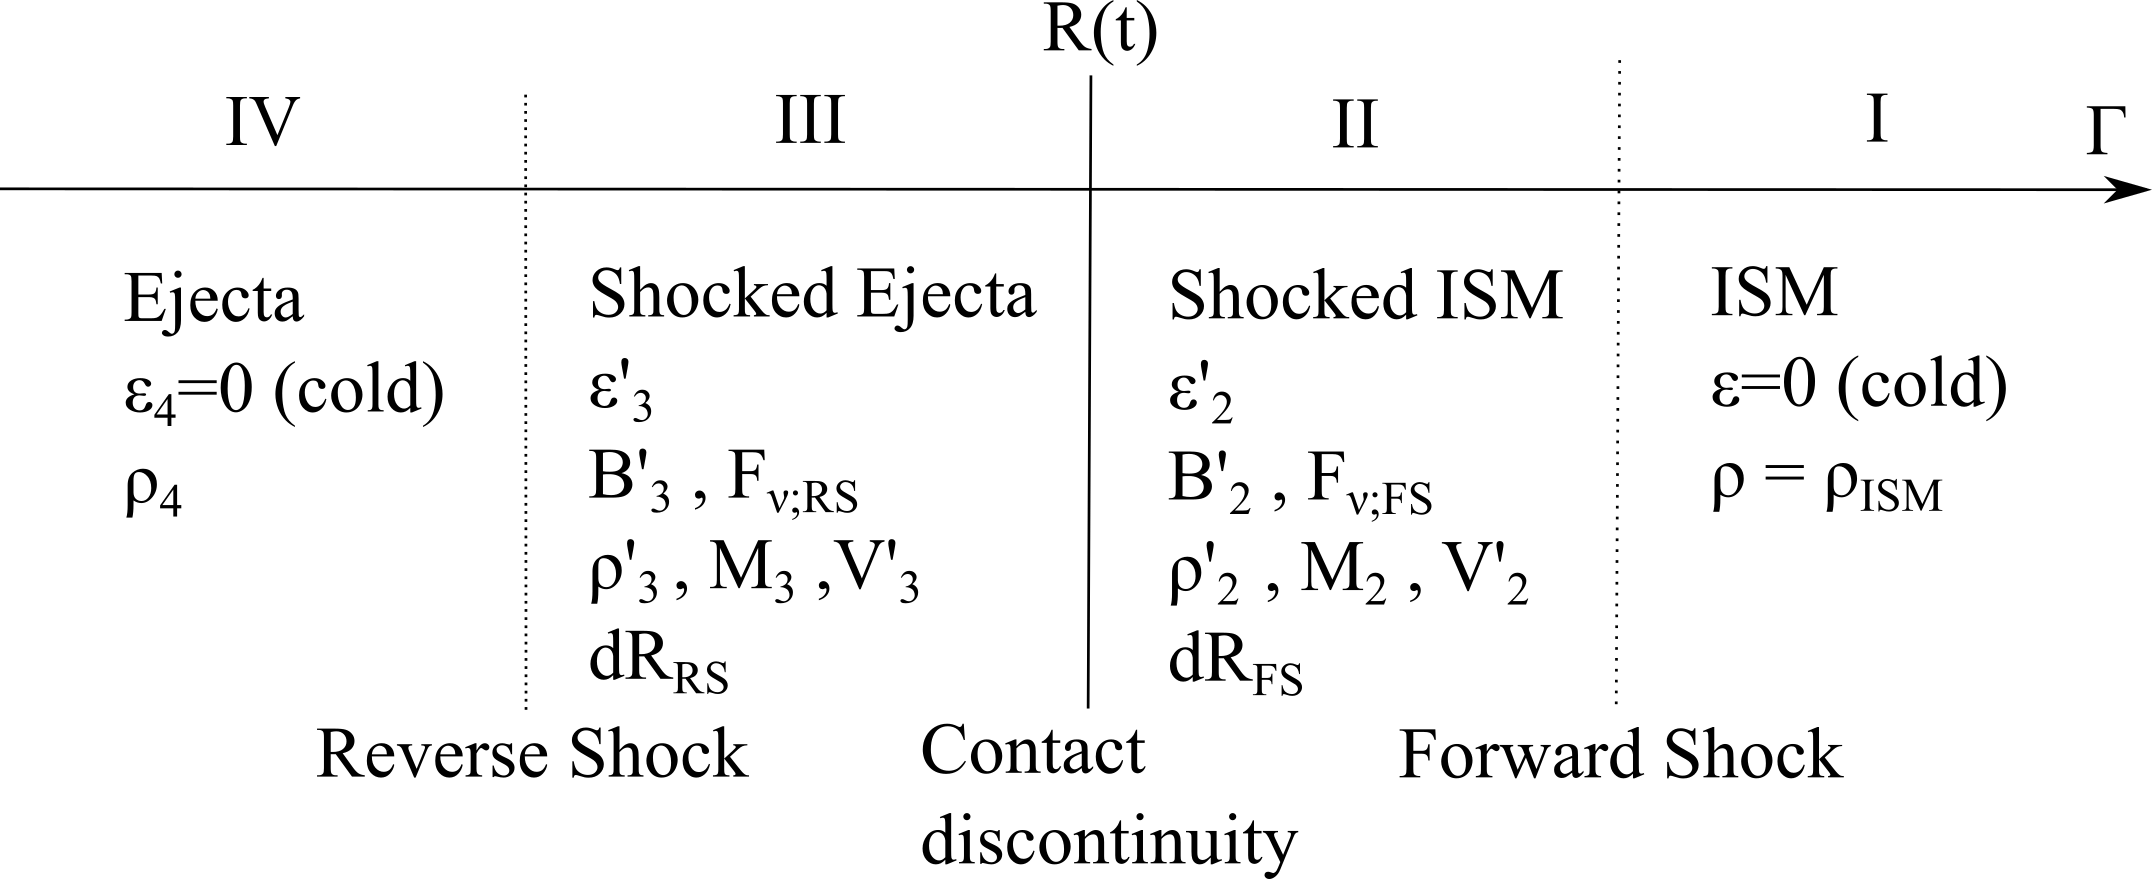
\includegraphics[height=3.0cm]{figures/blast_wave_struct.png}
            }};
        }
    \end{tikzpicture}
\end{frame}


% =============================================================================================

\subsection{Electron distribution in shock downstream}
\begin{frame}{}  %% ---------- Intro/motivation 
    \begin{tikzpicture}[overlay,remember picture]
        \uncover<1->{ % <-> |
            \node (t1) [anchor=center,scale=1,opacity=1] at ([shift={(-3.8cm,-0.2cm)}]current page.center){
                \parbox{0.5\textwidth}{
                    % power = energy/time/steradian/frequency
                    Fokker-Plank type equation:
%                    \begin{equation*}
%                        \frac{\partial}{\partial t}n_e(\gamma_e,t) = \frac{\partial}{\partial \gamma_e} \Bigg( -\frac{\sigma_T B^2}{6 \pi m_e c} \gamma_e^2 \Bigg) n_e(\gamma_e, t) + Q(\gamma)
%                    \end{equation*},
%                    where $Q(\gamma_e)\propto\gamma_e^{-p}$ with $\gamma_{m}\leq\gamma_e\leq\gamma_{\rm max}$ 
                    %
                    \begin{equation*}
                        \frac{\partial N(\gamma, t')}{\partial t'} = -\frac{\partial}{\partial \gamma}\Big[ \big( \dot{\gamma}_{\rm syn} + \dot{\gamma}_{\rm adi} N(\gamma, t') \big)  \Big] + Q(\gamma, t')
                    \end{equation*}
                    %
                    \begin{equation*}
                        \dot{\gamma}_{\rm syn} = - \frac{4}{3}\frac{\sigma_T c}{m_e c^2}\gamma^2, \hspace{3mm} \dot{\gamma}_{\rm adi} = -\frac{\gamma \beta_e^2}{3}\frac{d\ln V'}{dt'}, 
                    \end{equation*}
                    %
                    \begin{equation*}
                        Q(\gamma,t) = 
%                        \frac{dN_{\rm inj}}{dt d\gamma}=
                        \begin{cases}
                            Q_0(\gamma_m, t)\Big(\frac{\gamma}{\gamma_m}\Big)^{-p} & \gamma\in(\gamma_m,\gamma_M), \\
                            0 & \text{elswhere}.
                        \end{cases}
                    \end{equation*}
                    %
                    Steady state solution $\partial/\partial t' = 0$ and $\dot{\gamma}_{\rm adi} = 0$.
                    Cooling $\gamma_c = 6\pi m_e c / ( \sigma_T B^2 t )$.
                    
                    Electron cooling modifies distribution
                }};
            }
        \uncover<1->{ % <-> |
            \node (t1) [anchor=center,scale=1,opacity=1] at ([shift={(4.5cm,-0.5cm)}]current page.center){
                \parbox{0.45\textwidth}{
                    %
%                    \begin{equation*}
%                        \gamma_c = \frac{6\pi m_e c}{\sigma_T B^2 t}, 
%                    \end{equation*}
                    Electrons $\gamma > \gamma_c$ occupy $(\gamma/\gamma_c)^{-1}\ll 1$ fractional depth. 
                    Effective line-of-sight electron distribution
                    \begin{equation*}
                        \Big\langle \frac{\partial N}{\partial \gamma} \Big\rangle \propto  \frac{\partial N}{\partial \gamma}  \min \Big( 1, \frac{\gamma_c}{\gamma} \Big)
                    \end{equation*}
                    %
                    \begin{equation*}
                        \Big\langle \frac{\partial N}{\partial \gamma} \Big\rangle_{\rm fc} \propto
                        \begin{cases}
                            \gamma^{-p} & \gamma_m < \gamma < \gamma_c; \\
                            \gamma^{-p-1} & \gamma > \gamma_c
                        \end{cases}
                    \end{equation*}
                    %
                    \begin{equation*}
                        \Big\langle \frac{\partial N}{\partial \gamma} \Big\rangle_{\rm sc} \propto
                        \begin{cases}
                            \gamma^2 & \gamma_c < \gamma < \gamma_m; \\
                            \gamma^{-p-1} & \gamma > \gamma_m
                        \end{cases}
                    \end{equation*}
                    %
                    Afterglow spectrum is defined by $\gamma_m$ and $\gamma_c$
            }};
        }
        
    \end{tikzpicture}
\end{frame}

% =============================================================================================

\subsection{Cyclosynchrotron emission}
\begin{frame}{}  %% ---------- Intro/motivation 
    \begin{tikzpicture}[overlay,remember picture]
        \uncover<1->{ % <-> |
            \node (t1) [anchor=center,scale=1,opacity=1] at ([shift={(-0.0cm,-0.2cm)}]current page.center){
                \parbox{1.1\textwidth}{
                    % power = energy/time/steradian/frequency
                    \begin{equation*}
                        \boldsymbol{\eta}(\boldsymbol{\beta},\theta)d\omega = \frac{e^2 \omega^2}{2 \pi c}\Bigg[ \sum_{m=1}^{\infty} \Bigg( \frac{\cos\theta - \beta_{||}}{\sin \theta} \Bigg)^2 J_m^2(x) + \beta_{\perp}^2 J_m^{'2}(x) \Bigg]\delta(y) d\omega
                    \end{equation*}
                    where $x = (\omega/\omega_0)\beta_{\perp}\sin\theta$
                    $y=m\omega_0 - \omega(1 - \beta_{||}\cos\theta)$,
                    $\delta(y)$ is the delta function $J_m(x)$ is the Bessel function, 
                    $\beta_{||} = \beta\cos\theta_p$, $\beta_{\perp}=\beta\sin\theta_p$, 
                    with $\theta_p=\angle(\boldsymbol{\beta},\boldsymbol{B})$.
                    \begin{itemize}
                        \item Cyclotron, $m\beta \ll 1$: Expand $J(x)$ to lowest $x$, for successive harminics. 
                        \item Synchrotron $\gamma_e \gg 1$ : $J(x)$ approximated by modified Bessel function
                    \end{itemize}
                    \begin{equation*}
                        \frac{dE}{d\omega} = \frac{\sqrt{3}e^3 B \sin\theta_p}{2 \pi m_e c^2}
                        \frac{\omega}{\omega_c}\int_{\omega/\omega_c}^{\infty}F_{5/3}(\xi)d\xi,
                    \end{equation*}
                    where $\omega_c = (3/2) \gamma^2 \omega_b \sin \theta_p$
                    \begin{equation*}
                        L_{\omega} = 
%                        \frac{dE}{d\omega}=
                        2\pi\int_0^1 
%                        d\beta n(\beta) 
                        \frac{\partial N}{\partial \gamma_e} d\gamma_e
                        \int_0^1 d(\cos\theta_p) \int_{-1}^{1}d(\cos\theta)\boldsymbol{\eta}_{\boldsymbol{\beta},\theta}.
                    \end{equation*}
            }};
        }
        %        
        %        \uncover<1->{ % <-> |
            %            \node (t1) [anchor=center,scale=1,opacity=1] at ([shift={(0.0cm,-3.8cm)}]current page.center){
                %                \parbox{1.1\textwidth}{
                    %                    \red{Questions}: remnant's lifetime; ejecta properties; \rproc{} cites
                    %            }};
            %        }
        
    \end{tikzpicture}
\end{frame}

% =============================================================================================

\subsection{Synchrotron spectrum from non-thermal electrons}
\begin{frame}{}  %% ---------- Intro/motivation 
    \begin{tikzpicture}[overlay,remember picture]
        \uncover<1->{ % <-> |
            \node (t1) [anchor=center,scale=1,opacity=1] at ([shift={(0.8cm,2.2cm)}]current page.center){
                \parbox{1.0\textwidth}{
                    \begin{itemize}
                        \item (i) low-energy tail $\nu < \min(\nu_m, \nu_c)$,
                        \item (ii) power-law segment $\nu\in(\nu_m,\nu_c)$
                        \item (iii) exponential cut-off $\nu>\max(\nu_m,\nu_c)$
                    \end{itemize}
            }};
        }
        \uncover<1->{ % <-> |
            \node (img1) [anchor=center,scale=1,opacity=1] at ([shift={(-0.8cm,-1.5cm)}]current page.center){
                \parbox{1.0\textwidth}{
                    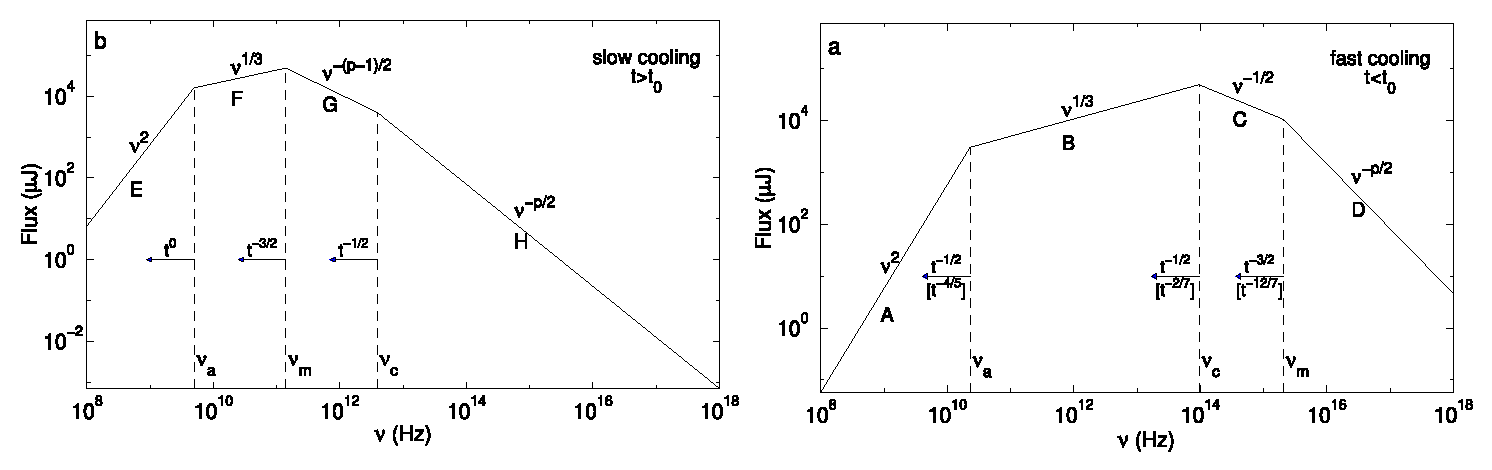
\includegraphics[height=5cm]{figures/sari97_flat.pdf}
            }};
        }
    \end{tikzpicture}
\end{frame}

% =============================================================================================

\subsection{Thermal electrons in mildly relativistic shocks}
\begin{frame}{}  %% ---------- Intro/motivation 
    \begin{tikzpicture}[overlay,remember picture]
        \uncover<1->{ % <-> |
            \node (t1) [anchor=center,scale=1,opacity=1] at ([shift={(-3.0cm,2.2cm)}]current page.center){
                \parbox{0.5\textwidth}{
                    \begin{itemize}
                        \item ``Thermal spectrum'' (left)
                        \item ``Non-thermal spectrum'' (right)
                    \end{itemize}
                $\beta_{\rm sh}=0.1$, $n_{\rm ISM}=10^4\,\ccm$, $t=200\,$d, $\delta=0.1$, $p=3$, $B=0.1\,$G, $\varepsilon_T=0.1$
            }};
        }
        \uncover<1->{ % <-> |
            \node (t1) [anchor=center,scale=1,opacity=1] at ([shift={(4.0cm,2.2cm)}]current page.center){
                \parbox{0.5\textwidth}{
                    \begin{eqnarray*}
                        \frac{\partial N}{\partial \gamma}\Big|_{\rm th} &= n_{e} \frac{ \gamma^2\sqrt{1-\gamma^{-2}} }{K_2(1/\Theta) \Theta} e^{-\gamma/\Theta}, \\
%                        \hspace{5mm}
                        \frac{\partial N}{\partial \gamma}\Big|_{\rm pl} &= n_e g(\Theta)\delta\frac{p-2}{3\Theta}\Big(\frac{\gamma}{3\Theta}\Big)^{-p}
                    \end{eqnarray*}
                    
                    
%                    Spectrum $3$ segments: 
%                    (i) $\nu < \nu_c$: low energy tail, $F_{\nu}\propto\nu^{1/3}$, 
%                    (ii) $\nu(\gamma) > \nu_c$ power law segment $F_{\nu}\propto\nu^{-1/2}$ 
%                    (iii) $\nu(\gamma)$and 
            }};
        }
        \uncover<1->{ % <-> |
            \node (img1) [anchor=center,scale=1,opacity=1] at ([shift={(2.cm,-1.5cm)}]current page.center){
                \parbox{1.0\textwidth}{
                    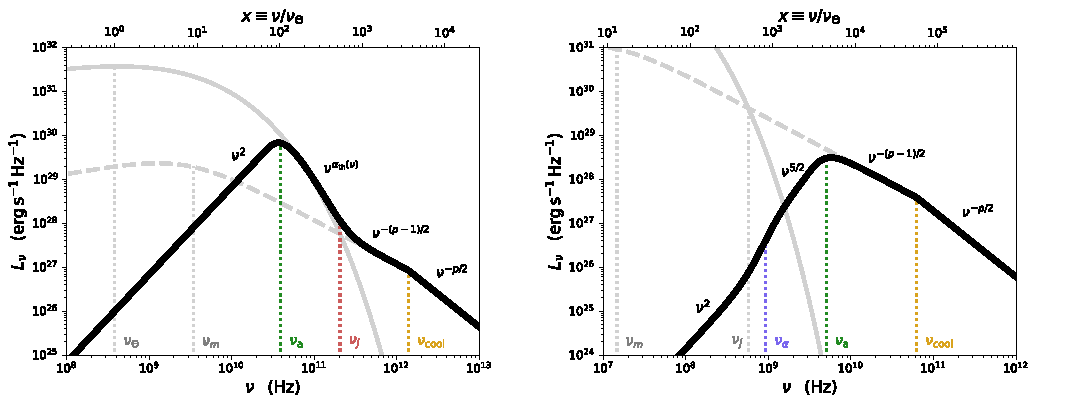
\includegraphics[height=5cm]{figures/Margalit21_thermalElectrons.pdf}
            }};
        }
    \end{tikzpicture}
\end{frame}

% =============================================================================================

\section{Preliminary Results}
\subsection{Modelling sGRB afterglow (GRB170817A)}
\begin{frame}{}  %% ---------- Intro/motivation 
    \begin{tikzpicture}[overlay,remember picture]
         \uncover<1->{ % <-> |
            \node (t1) [anchor=center,scale=1,opacity=1] at ([shift={(-3.0cm,2.5cm)}]current page.center){
                \parbox{0.7\textwidth}{
                    \begin{itemize}
                        \item Gaussian jet $E(\theta) \propto e^{(\theta/\theta_c)^2}$
                        \item Off-axis $\theta_{\rm obs} > \theta_c$
                        \item Relativistic core, $\Gamma_c \sim 10^2$; low ISM density.
                    \end{itemize}
            }};
        }
        \uncover<1->{ % <-> |
            \node (img1) [anchor=center,scale=1,opacity=1] at ([shift={(1.cm,-1.35cm)}]current page.center){
                \parbox{1.0\textwidth}{
                    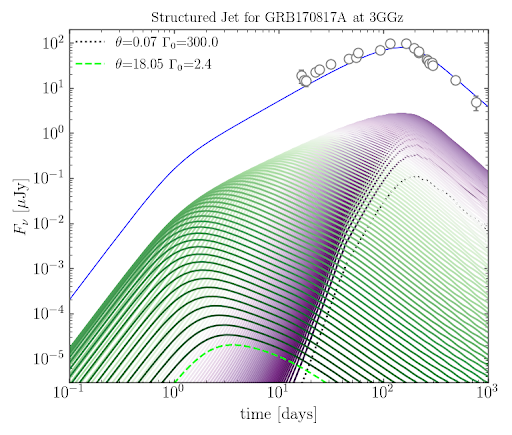
\includegraphics[height=6cm]{figures/grb170817fernandezPyBlastAfterglow.png}
            }};
        }
        \uncover<1->{ % <-> |
            \node (img1) [anchor=center,scale=1,opacity=1] at ([shift={(9.0cm,-0.5cm)}]current page.center){
                \parbox{1.0\textwidth}{
                    Flux centroid motion, $4.5\,$GGz; \\
                    Color is $I/I_{\rm max}$ %is shown with $I=0.01I_{\rm max}$ cut
                    
                    \movie[width=0.8\textwidth]{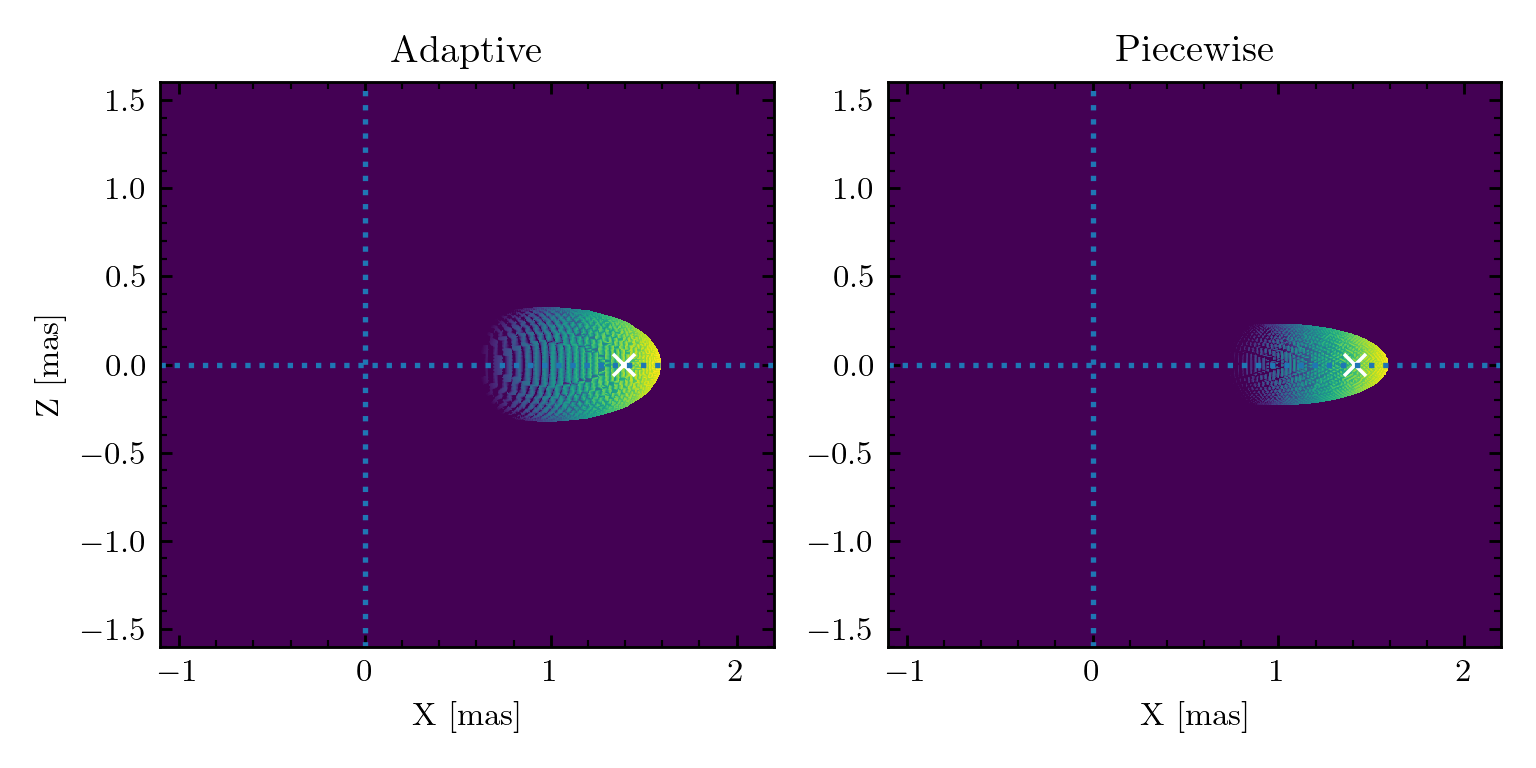
\includegraphics[width=0.8\textwidth]{figures/200.png}}{figures/out2.mp4}
            }};
        }
    \end{tikzpicture}
\end{frame}

% =============================================================================================

\subsection{Extracting kilonova ejecta profile}
\begin{frame}{}  %% ---------- Intro/motivation 
    \begin{tikzpicture}[overlay,remember picture]
        \uncover<1->{ % <-> |
            \node (t1) [anchor=center,scale=1,opacity=1] at ([shift={(-3.0cm,2.5cm)}]current page.center){
                \parbox{0.7\textwidth}{
                    \begin{itemize}
                        \item $E_{\rm k} = f(\theta,\beta)$
                        \item $E_{\rm k;max}$ at $\theta\rightarrow0$ and $\beta\rightarrow0.2$.
                        \item $\log_{10}(E_k)=b_0 + (b_1 \theta) + (b_2 \beta) + (b_3 \theta^2) + (b_4 \theta \beta) + (b_5 \beta^{1/4})$
                    \end{itemize}
            }};
        }
        \uncover<1->{ % <-> |
            \node (img1) [anchor=center,scale=1,opacity=1] at ([shift={(2.2cm,-1.35cm)}]current page.center){
                \parbox{1.0\textwidth}{
                    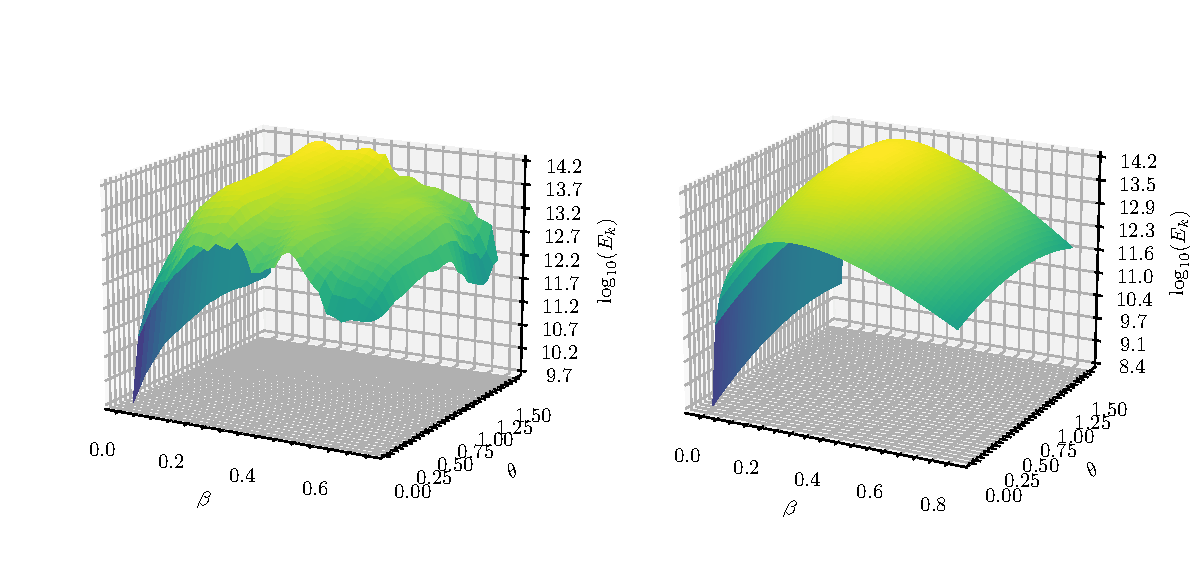
\includegraphics[height=6cm]{figures/fit_2d_ejecta.pdf}
            }};
        }
        \uncover<1->{ % <-> |
            \node (img1) [anchor=center,scale=1,opacity=1] at ([shift={(9cm,2cm)}]current page.center){
                \parbox{1.0\textwidth}{
                    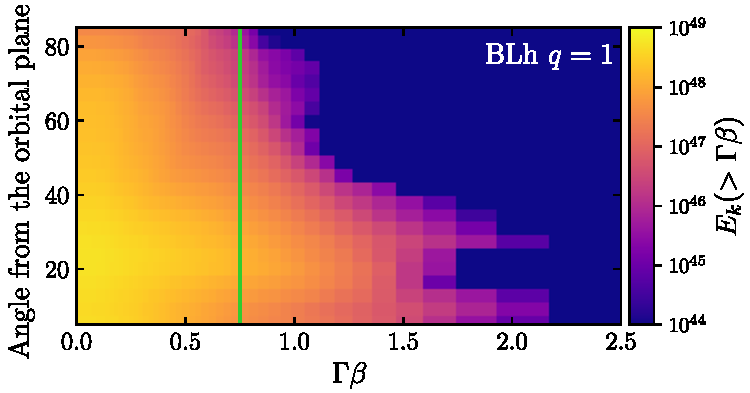
\includegraphics[height=3cm]{figures/kinetic_energy_struct_models_bottom_only.pdf}
            }};
        }
    \end{tikzpicture}
\end{frame}
